% Options for packages loaded elsewhere
\PassOptionsToPackage{unicode}{hyperref}
\PassOptionsToPackage{hyphens}{url}
%
\documentclass[
  ignorenonframetext,
  aspectratio=169]{beamer}
\usepackage{pgfpages}
\setbeamertemplate{caption}[numbered]
\setbeamertemplate{caption label separator}{: }
\setbeamercolor{caption name}{fg=normal text.fg}
\beamertemplatenavigationsymbolsempty
% Prevent slide breaks in the middle of a paragraph
\widowpenalties 1 10000
\raggedbottom
\setbeamertemplate{part page}{
  \centering
  \begin{beamercolorbox}[sep=16pt,center]{part title}
    \usebeamerfont{part title}\insertpart\par
  \end{beamercolorbox}
}
\setbeamertemplate{section page}{
  \centering
  \begin{beamercolorbox}[sep=12pt,center]{part title}
    \usebeamerfont{section title}\insertsection\par
  \end{beamercolorbox}
}
\setbeamertemplate{subsection page}{
  \centering
  \begin{beamercolorbox}[sep=8pt,center]{part title}
    \usebeamerfont{subsection title}\insertsubsection\par
  \end{beamercolorbox}
}
\AtBeginPart{
  \frame{\partpage}
}
\AtBeginSection{
  \ifbibliography
  \else
    \frame{\sectionpage}
  \fi
}
\AtBeginSubsection{
  \frame{\subsectionpage}
}
\usepackage{amsmath,amssymb}
\usepackage{lmodern}
\usepackage{ifxetex,ifluatex}
\ifnum 0\ifxetex 1\fi\ifluatex 1\fi=0 % if pdftex
  \usepackage[T1]{fontenc}
  \usepackage[utf8]{inputenc}
  \usepackage{textcomp} % provide euro and other symbols
\else % if luatex or xetex
  \usepackage{unicode-math}
  \defaultfontfeatures{Scale=MatchLowercase}
  \defaultfontfeatures[\rmfamily]{Ligatures=TeX,Scale=1}
\fi
\usetheme[]{metropolis}
% Use upquote if available, for straight quotes in verbatim environments
\IfFileExists{upquote.sty}{\usepackage{upquote}}{}
\IfFileExists{microtype.sty}{% use microtype if available
  \usepackage[]{microtype}
  \UseMicrotypeSet[protrusion]{basicmath} % disable protrusion for tt fonts
}{}
\makeatletter
\@ifundefined{KOMAClassName}{% if non-KOMA class
  \IfFileExists{parskip.sty}{%
    \usepackage{parskip}
  }{% else
    \setlength{\parindent}{0pt}
    \setlength{\parskip}{6pt plus 2pt minus 1pt}}
}{% if KOMA class
  \KOMAoptions{parskip=half}}
\makeatother
\usepackage{xcolor}
\IfFileExists{xurl.sty}{\usepackage{xurl}}{} % add URL line breaks if available
\IfFileExists{bookmark.sty}{\usepackage{bookmark}}{\usepackage{hyperref}}
\hypersetup{
  pdfauthor={Olivier Gimenez},
  hidelinks,
  pdfcreator={LaTeX via pandoc}}
\urlstyle{same} % disable monospaced font for URLs
\newif\ifbibliography
\usepackage{longtable,booktabs,array}
\usepackage{calc} % for calculating minipage widths
\usepackage{caption}
% Make caption package work with longtable
\makeatletter
\def\fnum@table{\tablename~\thetable}
\makeatother
\usepackage{graphicx}
\makeatletter
\def\maxwidth{\ifdim\Gin@nat@width>\linewidth\linewidth\else\Gin@nat@width\fi}
\def\maxheight{\ifdim\Gin@nat@height>\textheight\textheight\else\Gin@nat@height\fi}
\makeatother
% Scale images if necessary, so that they will not overflow the page
% margins by default, and it is still possible to overwrite the defaults
% using explicit options in \includegraphics[width, height, ...]{}
\setkeys{Gin}{width=\maxwidth,height=\maxheight,keepaspectratio}
% Set default figure placement to htbp
\makeatletter
\def\fps@figure{htbp}
\makeatother
\setlength{\emergencystretch}{3em} % prevent overfull lines
\providecommand{\tightlist}{%
  \setlength{\itemsep}{0pt}\setlength{\parskip}{0pt}}
\setcounter{secnumdepth}{-\maxdimen} % remove section numbering
% Allowing for slides with 2 columns
\def\begincols{\begin{columns}[c]}
\def\endcols{\end{columns}}
\def\begincol{\begin{column}{0.5\textwidth}}
\def\endcol{\end{column}}

% Reducing black space between R code and output
% \setlength{\topsep}{0pt}{}
\setlength{\emergencystretch}{0em}
\setlength{\parskip}{2pt}
\setlength{\partopsep}{1pt}

% Reducing font size of R code and output
% Code below from http://stackoverflow.com/a/38324868
% See also http://stackoverflow.com/a/39961605

% Change fontsize of R code
\let\oldShaded\Shaded
\let\endoldShaded\endShaded
\renewenvironment{Shaded}{\footnotesize\oldShaded}{\endoldShaded}

% Change fontsize of output
\let\oldverbatim\verbatim
\let\endoldverbatim\endverbatim
\renewenvironment{verbatim}{\footnotesize\oldverbatim}{\endoldverbatim}
\ifluatex
  \usepackage{selnolig}  % disable illegal ligatures
\fi

\title{Bayesian statistics with R\\
3. Analyses by hand}
\author{Olivier Gimenez}
\date{November 2021}

\begin{document}
\frame{\titlepage}

\hypertarget{back-to-bayes}{%
\section{Back to Bayes}\label{back-to-bayes}}

\begin{frame}{A simple example}
\protect\hypertarget{a-simple-example}{}
\begin{itemize}
\tightlist
\item
  Let us take a simple example to fix ideas.
\item
  120 deer were radio-tracked over winter.
\item
  61 close to a plant, 59 far from any human activity.
\item
  Question: is there a treatment effect on survival?
\end{itemize}

\begin{longtable}[]{@{}lllll@{}}
\toprule
& Released & Alive & Dead & Other \\
\midrule
\endhead
treatment & 61 & 19 & 38 & 4 \\
control & 59 & 21 & 38 & 0 \\
\bottomrule
\end{longtable}
\end{frame}

\begin{frame}
\begin{itemize}[<+->]
\tightlist
\item
  So, \(n = 57\) deer were assigned to the treatment group of which
  \(k=19\) survived the winter.
\end{itemize}

\begin{itemize}[<+->]
\tightlist
\item
  Of interest is the probability of over-winter survival, call it
  \(\theta\), for the general population within the treatment area.
\end{itemize}

\begin{itemize}[<+->]
\tightlist
\item
  The obvious estimate is simply to take the ratio \(k/n=19/57\).
\end{itemize}

\begin{itemize}[<+->]
\tightlist
\item
  How would the classical statistician justify this estimate?
\end{itemize}
\end{frame}

\begin{frame}
\begin{itemize}
\tightlist
\item
  Our model is that we have a Binomial experiment (assuming independent
  and identically distributed draws from the population).
\end{itemize}

\pause

\begin{itemize}
\tightlist
\item
  \(K\) the number of alive individuals at the end of the winter, so
  that \(P(K=k) = \binom{n}{k}\theta^k(1-\theta)^{n-k}\).
\end{itemize}

\pause

\begin{itemize}
\tightlist
\item
  The classical approach is to maximise the corresponding likelihood
  with respect to \(\theta\) to obtain the entirely plausible MLE:
\end{itemize}

\[ \hat{\theta} = k/n = 19/57\].
\end{frame}

\begin{frame}{The Bayesian approach}
\protect\hypertarget{the-bayesian-approach}{}
\begin{itemize}[<+->]
\tightlist
\item
  The Bayesian starts off with a prior.
\end{itemize}

\begin{itemize}[<+->]
\tightlist
\item
  Now, the one thing we know about \(\theta\) is that is a continuous
  random variable and that it lies between zero and one.
\end{itemize}

\begin{itemize}[<+->]
\tightlist
\item
  Thus, a suitable prior distribution might be the Beta defined on
  \([0,1]\).
\end{itemize}

\begin{itemize}[<+->]
\tightlist
\item
  What is the Beta distribution?
\end{itemize}
\end{frame}

\begin{frame}{What is the Beta distribution?}
\protect\hypertarget{what-is-the-beta-distribution}{}
\[
q(\theta \mid \alpha, \beta) = \frac{1}{\text{Beta}(\alpha, \beta)}{\theta^{\alpha - 1}} {(1-\theta)^{\beta - 1}} 
\]

with
\(\text{Beta}(\alpha, \beta) = \displaystyle{\frac{\Gamma(\alpha)\Gamma(\beta)}{\Gamma(\alpha+\beta)}}\)
and \(\Gamma(n) = (n-1)!\)
\end{frame}

\begin{frame}
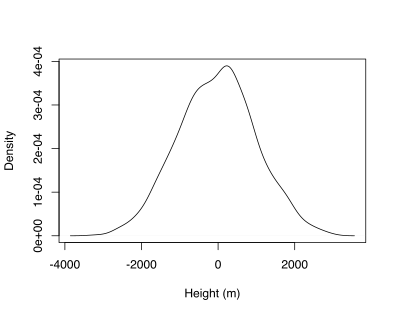
\includegraphics{example_files/figure-beamer/unnamed-chunk-1-1.pdf}
\end{frame}

\begin{frame}{The Bayesian approach}
\protect\hypertarget{the-bayesian-approach-1}{}
\begin{itemize}
\tightlist
\item
  We assume a priori that \(\theta \sim Beta(a,b)\) so that
  \(\Pr(\theta) = \theta^{a-1} (1 - \theta)^{b-1}\)
\end{itemize}

\pause

\begin{itemize}
\tightlist
\item
  Then we have:
\end{itemize}

\[
\begin{aligned}
{\color{red}{Pr(\theta \mid k)}} & \propto {\color{blue}{\binom{n}{k}\theta^k(1-\theta)^{n-k}}} \; {\color{green}{\theta^{a-1} (1 - \theta)^{b-1}}}\\
& \propto {\theta^{(a+k)-1}} {(1-\theta)^{(b+n-k)-1}} 
\end{aligned}
\]

\pause

\begin{itemize}
\tightlist
\item
  That is:
\end{itemize}

\[ \theta \mid k \sim Beta(a+k,b+n-k)\]

\pause

\begin{itemize}
\tightlist
\item
  Take a Beta prior with a Binomial likelihood, you get a Beta posterior
  (conjugacy)
\end{itemize}
\end{frame}

\begin{frame}{Application to the deer example}
\protect\hypertarget{application-to-the-deer-example}{}
\begin{itemize}[<+->]
\tightlist
\item
  Posterior distribution of survival is \(\theta \sim Beta(a+k,b+n-k)\).
\end{itemize}

\begin{itemize}[<+->]
\tightlist
\item
  If we take a Uniform prior, i.e.~\(Beta(1,1)\), then we have:
\end{itemize}

\begin{itemize}[<+->]
\tightlist
\item
  \(\theta_{treatment} \sim Beta(1+19,1+57-19)=Beta(20,39)\)
\end{itemize}

\begin{itemize}[<+->]
\tightlist
\item
  Note that in this specific situation, the posterior has an explicit
  expression, easy to manipulate.
\end{itemize}

\begin{itemize}[<+->]
\tightlist
\item
  In particular, \(E(Beta(a,b)) = \displaystyle{\frac{a}{a+b}} = 20/59\)
  to be compared with the MLE \(19/57\).
\end{itemize}
\end{frame}

\begin{frame}{A general result}
\protect\hypertarget{a-general-result}{}
\textbf{This is a general result, the Bayesian and frequentist estimates
will always agree if there is sufficient data, so long as the likelihood
is not explicitly ruled out by the prior.}
\end{frame}

\begin{frame}{Prior \(Beta(1,1)\) and posterior survival
\(Beta(20,39)\)}
\protect\hypertarget{prior-beta11-and-posterior-survival-beta2039}{}
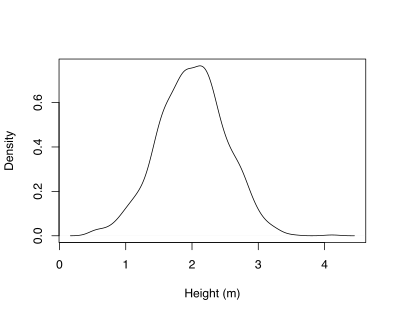
\includegraphics{example_files/figure-beamer/unnamed-chunk-2-1.pdf}
\end{frame}

\begin{frame}{Prior \(Beta(1,1)\) and posterior survival
\(Beta(20,39)\)}
\protect\hypertarget{prior-beta11-and-posterior-survival-beta2039-1}{}
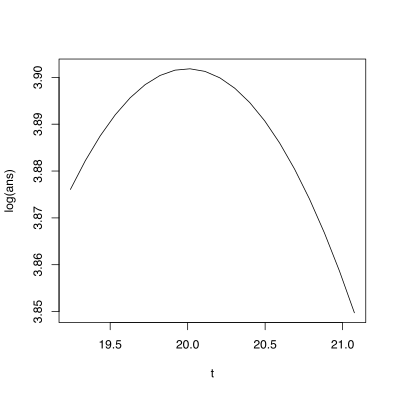
\includegraphics{example_files/figure-beamer/unnamed-chunk-3-1.pdf}
\end{frame}

\begin{frame}{Notation}
\protect\hypertarget{notation}{}
Our model so far

\begin{align*}
   y &\sim \text{Binomial}(N, \theta) &\text{[likelihood]}
   \\
  \theta &\sim \text{Beta}(1, 1) &\text{[prior for }\theta \text{]} \\ 
\end{align*}
\end{frame}

\begin{frame}
\includegraphics{img/bayes_puppies.png}
\end{frame}

\end{document}
